\section{Experiments}
\label{sec:exp}

\begin{figure*}[t]
    \centering
    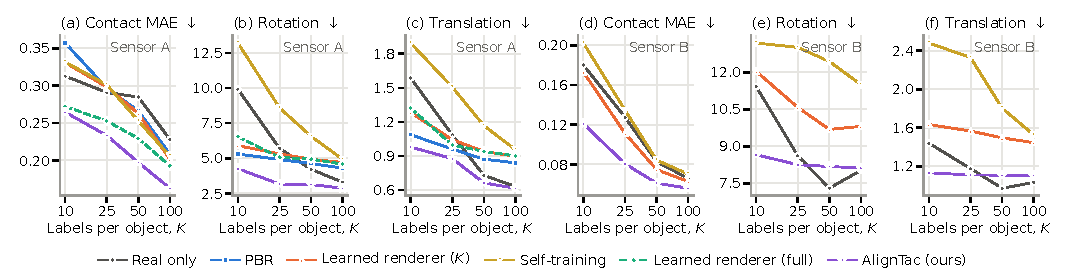
\includegraphics[width=0.9\textwidth]{figures/fig_kshot.pdf}
    \caption{\textbf{Label efficiency on two tactile sensors.} $K$: labeled training contacts per object. (a--c) Sensor-A validation, 150 epochs; the all-pairs (leaky) reference uses extra real labels and 50 epochs at $K=10$. (d--f) Sensor-B test, 50 epochs, renderer-free MeshTac. Matched methods share the registered contacts.}
    \label{fig:kshot}
\end{figure*}

\begin{table}[!htb]
\centering
\tableformat
\setlength{\tabcolsep}{3.0pt}
\begin{tabularx}{\columnwidth}{@{}rXrrrr@{}}
\toprule
$\Kreal$ & Method & \metrichead{Depth}{MSE} & \metrichead{Contact}{MAE} & \shortstack[c]{\strut IoU\\\strut $\uparrow$} & \metrichead{Rot.}{(deg)} \\
\midrule
\tabkshotshort
\bottomrule
\end{tabularx}
\caption{\textbf{Label-budget comparison on sensor A.} Validation: $472$ frames; $K$ labels per object. Self-training and MeshTac also use unlabeled images. Italic all-pairs rows exceed the budget ($K=10$: 50 epochs; others: 150). Matched rows use 150 epochs; bold marks the best at each $K$.}
\label{tab:kshot}
\end{table}

\subsection{Label Efficiency}
\label{sec:kshot}
We compare real-only training, learned-renderer augmentation, teacher-depth self-training and MeshTac using the same registered contacts at each $K$ (Table~\ref{tab:kshot}, Fig.~\ref{fig:kshot}). Self-training and MeshTac receive the same unlabeled training images; self-training applies pose supervision only to the registered subset.

At $K=25$, MeshTac lowers depth MSE by $19\%$ and contact MAE by $20\%$ relative to real-only training. Synthetic augmentation slightly improves all-pixel MSE but worsens contact MAE and IoU: lower MSE need not mean better contact reconstruction when background pixels dominate. Three-seed comparisons at 50 epochs confirm the MeshTac gain. MeshTac at $K=50$ also outperforms real-only training at $K=100$ in depth MSE ($0.0307$ versus $0.0369$), showing the value of aligned contacts beyond the registered set.

Removing the renderer preserves the depth improvement at every budget, supporting alignment as the main source of the within-session gain. Synthetic augmentation becomes useful for contact reconstruction at $K\ge50$ and under session changes (Sec.~\ref{sec:general}). Rotation improves for $K\le50$ but not at $K=100$; the reconstruction gain does not extend uniformly to pose.

\begin{table}[!htb]
\centering
\tableformat
\setlength{\tabcolsep}{1.8pt}
\resizebox{\columnwidth}{!}{%
\begin{tabular}{@{}lrrrrrrr@{}}
\toprule
& \multicolumn{3}{c}{Pseudo-labels vs.\ GT} & \multicolumn{4}{c}{Student validation} \\
\cmidrule(lr){2-4}\cmidrule(lr){5-8}
Pseudo-label & \shortstack[c]{\strut IoU\\\strut $\uparrow$} & \metrichead{Cont.}{MAE} & \metrichead{Rot.}{(deg)} & \metrichead{Depth}{MSE} & \metrichead{Cont.}{MAE} & \shortstack[c]{\strut IoU\\\strut $\uparrow$} & \metrichead{Rot.}{(deg)} \\
\midrule
\tabrcablmain
\bottomrule
\end{tabular}}
\caption{\textbf{Pseudo-label quality and student performance.} Sensor A, $K=25$, 50 epochs. Student results are three-seed means except \emph{Teacher depth + pose}. Withheld training GT scores labels only. $^{1/2}$ uses mesh depth for each object's half with lowest render error, teacher depth otherwise, and L1-search pose throughout. $\ddagger$ removes the renderer throughout the pipeline.}
\label{tab:abl}
\end{table}

\begin{figure}[t]
    \centering
    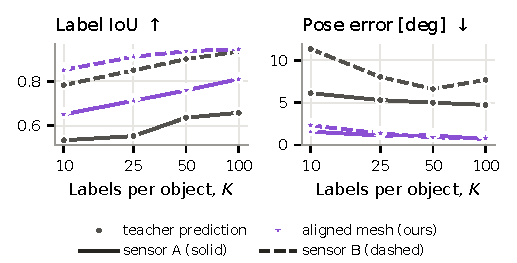
\includegraphics[width=\columnwidth]{figures/fig_labels.pdf}
    \caption{\textbf{Teacher and aligned-mesh label quality.} IoU, contact MAE and rotation error on unlabeled training images from both sensors, across label budgets $K$. Withheld GT is used only to evaluate the labels.}
    \label{fig:labels}
\end{figure}

\subsection{Ablation Study on Alignment Quality}
\label{sec:ablation}
We label the same unlabeled images with teacher predictions, L1 render-and-compare search or learned alignment, then evaluate both label quality and the student trained on those targets (Table~\ref{tab:abl}). Adding teacher pose isolates pose supervision; the renderer-free row additionally removes synthetic data.

Adding teacher pose mainly improves student rotation. Learned alignment improves label quality on both sensors (Fig.~\ref{fig:labels}) and raises student IoU from $0.624$ to $0.729$ relative to teacher-depth self-training. Correcting mesh placement therefore improves the supervision supplied to the student.

L1 search gives smaller gains. At $K=25$, the renderer assigns lower image error to the search-selected pose than to the GT pose on $93\%$ of frames. Thus, image similarity can favor a geometrically incorrect state; this statistic measures candidate ranking, not the search's pose-failure rate.

Gains persist with varied aligner settings and two random label selections; a second labeling round adds little. At $K=25$, $1.6\%$ of aligned sensor-A training poses exceed $5^\circ$ error, mostly on one nearly symmetric object. Translation errors follow repeated ridges, where different states can yield similar contact geometry.

\begin{figure*}[t]
    \centering
    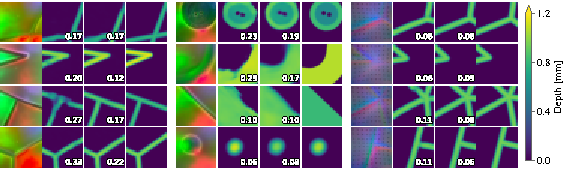
\includegraphics[width=0.8\textwidth]{figures/fig_qual.pdf}
    \caption{\textbf{Contact-depth reconstruction at $K=25$.} Each sensor shows three objects; each frame has its object's median contact-MAE improvement over real-only training. Numbers are contact MAE (mm), and depth maps share a color scale. Both displayed MeshTac models use synthetic data; the sensor-B curves in Fig.~\ref{fig:kshot}d--f use the renderer-free variant.}
    \label{fig:qual}
\end{figure*}

\begin{table}[!htb]
\centering
\tableformat
\setlength{\tabcolsep}{3pt}
\begin{tabularx}{\columnwidth}{@{}rXrr@{}}
\toprule
\multicolumn{4}{l}{\textbf{Sensor A: second-session evaluation}} \\
$\Kreal$ & Method & \metrichead{Contact}{MAE} & \shortstack[c]{\strut IoU\\\strut $\uparrow$} \\
\midrule
\tabcrossshortb
\midrule\midrule
\multicolumn{4}{l}{\textbf{Sensor B: sensor-specific training}} \\
$\Kreal$ & Method & \metrichead{Contact}{MAE} & \shortstack[c]{\strut IoU\\\strut $\uparrow$} \\
\midrule
\tabsbshortb
\bottomrule
\end{tabularx}
\caption{\textbf{Second-session and second-sensor results.} Top: sensor-A models tested on session 2 without retraining ($854$ frames). $\dagger$ uses all training labels from nine objects, with different object coverage from the $K$-shot rows. Bottom: models trained on sensor B and evaluated on its test set ($1{,}620$ frames); MeshTac is renderer-free. Sensor-B values are three-seed mean $\pm$ standard deviation. Contact MAE is in mm.}
\label{tab:general}
\end{table}

\subsection{Generalization Across Sessions and Sensors}
\label{sec:general}
\noindent\textbf{Second session.} We test sensor-A models on another day's contacts after object re-placement, without retraining (Table~\ref{tab:general}, top). MeshTac lowers contact MAE by $16\%$ at $K=25$ and $28\%$ at $K=100$ relative to real-only training. At $K=100$, synthetic augmentation improves on renderer-free MeshTac, which still outperforms self-training. At $K=25$, removing it gives slightly lower MAE ($0.306$ versus $0.310$). The benefit of simulation under this session change thus depends on the label budget.

\noindent\textbf{Second sensor.} We train each method separately on sensor B, keeping the aligner settings unchanged (Table~\ref{tab:general}, bottom). Renderer-free MeshTac lowers contact MAE by $36\%$ at $K=25$ and matches real-only training with twice as many labels. Three-seed checks at every budget support the gain, and evaluation with the original public labels gives the same qualitative result. At the other budgets, MeshTac lowers contact MAE by $15$--$33\%$, compared with at most $10\%$ from learned-renderer augmentation and no gain from self-training (Fig.~\ref{fig:kshot}e).

Figure~\ref{fig:qual} illustrates differences in ridge continuity and junction placement; quantitative comparisons use all evaluation frames.

\begin{table}[!htb]
\centering
\tableformat
\setlength{\tabcolsep}{3.5pt}
\begin{tabular}{@{}rrrrrrrrr@{}}
\toprule
& \multicolumn{4}{c}{Validation (session 1)} & \multicolumn{4}{c}{Session 2} \\
\cmidrule(lr){2-5}\cmidrule(lr){6-9}
& \multicolumn{2}{c}{Real only} & \multicolumn{2}{c}{MeshTac} & \multicolumn{2}{c}{Real only} & \multicolumn{2}{c}{MeshTac} \\
$\Kreal$ & pred. & +align & pred. & +align & pred. & +align & pred. & +align \\
\midrule
\tabposeref
\bottomrule
\end{tabular}
\caption{\textbf{Rotation error before and after mesh-assisted refinement.} Sensor A, mean error (deg) on session-1 validation and session-2 test images. \emph{pred.}: predictor output; \emph{+align}: six fixed-aligner iterations, without retraining.}
\label{tab:poseref}
\end{table}

\subsection{Mesh-Assisted Test-Time Pose Refinement}
\label{sec:tta}
We apply six fixed-aligner updates to real-only and MeshTac predictions using the test image and known mesh (Table~\ref{tab:poseref}). At $K\ge25$, both initializations reach $0.4$--$1.2^\circ$ mean rotation error within session 1: the aligner remains useful after student training and with a different predictor. At these budgets, session-2 means near $5^\circ$ exceed medians of $1.5$--$1.8^\circ$, motivating a confidence estimate to detect large residual errors.

\begin{table}[!htb]
\centering
\tableformat
\begin{tabularx}{\columnwidth}{Xrrrr}
\toprule
Method & \metrichead{Depth}{MSE} & \metrichead{Contact}{MAE} & \shortstack[c]{\strut IoU\\\strut $\uparrow$} & \metrichead{Rot.}{(deg)} \\
\midrule
\tabloomain
\bottomrule
\end{tabularx}
\caption{\textbf{Renderer baselines on held-out objects.} Sensor A, $1{,}244$ frames from three objects. Matched methods exclude their real contacts from training; simulation can use their meshes, except in the \emph{w/o held-out meshes} control. The italic leaky reference also uses real training pairs from these objects. Bold marks the best matched result.}
\label{tab:loo}
\end{table}

\subsection{Renderer Baselines: Unseen Objects and Label Leakage}
\label{sec:study}
We remove three objects from real training while allowing simulation to use their meshes (Table~\ref{tab:loo}). A control excludes those meshes as well. Simulated contacts lower rotation error from $64.7^\circ$ to $5$--$7^\circ$; removing the held-out meshes largely removes this gain. Dense MSE improves by at most $13\%$ among matched methods. In this setting, simulation provides more effective supervision for unseen-object pose than for dense reconstruction.

We then compare renderers trained on the same $K$ registered contacts with the all-pairs reference. The latter lowers MSE by $24$--$26\%$ in the few-label regime, but has access to additional real training labels. It represents a larger supervision budget; validation images remain excluded. Across 14 matched settings, contact-region image L1 correlates with downstream MSE ($\rho=0.95$). This supports its use for screening renderers, although the pooled correlation across budgets and variants does not establish causality or replace downstream evaluation.
